\documentclass[aspectratio=169]{beamer}

\usetheme{Madrid}
\usecolortheme{seahorse}
\setbeamertemplate{navigation symbols}{}
\setbeamertemplate{footline}[frame number]

\usepackage{amsmath}
\usepackage{tikz}
\usetikzlibrary{arrows.meta,positioning}

\begin{document}

% Speech note:
% Good morning everyone. Today I am going to introduce my project,
% "Incremental Data-Driven Robust Crew Pairing Optimization Under Evolving
% Uncertainty." The project is about airline crew pairing, which means deciding
% which crews should cover which flights. This is difficult because flights can
% be delayed, and a small delay can affect many later connections.
% The main problem is uncertainty. Traditional planning often depends on fixed
% assumptions or fitted probability distributions, but real disruptions are not
% always well described by those models. My project uses historical delay data
% to build one-sided delay bounds, because late arrivals hurt the schedule while
% early arrivals usually do not. A budget-of-uncertainty parameter controls how
% conservative the plan should be, so the model protects against serious delays
% without assuming every flight is delayed at the same time.
\begin{frame}{Project Overview}
  \begin{center}
    {\Large \textbf{Incremental Data-Driven Robust Crew Pairing Optimization}}\\
    \vspace{0.08cm}
    {\small Under Evolving Uncertainty}\\
    \vspace{0.12cm}
    {\small Xinyu Huang}
  \end{center}

  \vspace{0.15cm}
  \begin{columns}[T,onlytextwidth]
    \column{0.48\textwidth}
      \textbf{Problem}
      \begin{itemize}
        \item Airline crew schedules must cover all flights.
        \item Delays can break planned crew connections.
        \item Historical data may miss rare but important disruptions.
      \end{itemize}

    \column{0.48\textwidth}
      \textbf{Main idea}
      \begin{itemize}
        \item Build delay bounds from empirical quantiles.
        \item Model only harmful one-sided disruptions.
        \item Use a budget parameter to balance robustness and cost.
      \end{itemize}
  \end{columns}

  \vspace{0.25cm}
  \[
    \hat{\mathcal U}(\Gamma)
    =
    \left\{\Delta: 0 \le \Delta_f \le d_f,\;
    \sum_f \Gamma_f \le \Gamma,\;
    \Delta_f = \Gamma_f d_f \right\}
  \]
\end{frame}

% Speech note:
% The solution is a two-stage robust optimization model. In the first stage,
% the airline selects crew pairings before the disruption is known. In the
% second stage, after a delay scenario appears, the model chooses recovery
% actions such as waiting, swapping, or cancelling. To solve the model, the
% project combines nested column-and-constraint generation with column
% generation. This helps the algorithm add only the most important disruption
% scenarios and only useful crew pairings, instead of trying to enumerate
% everything from the start.
\begin{frame}{Solution Framework}
  \begin{center}
  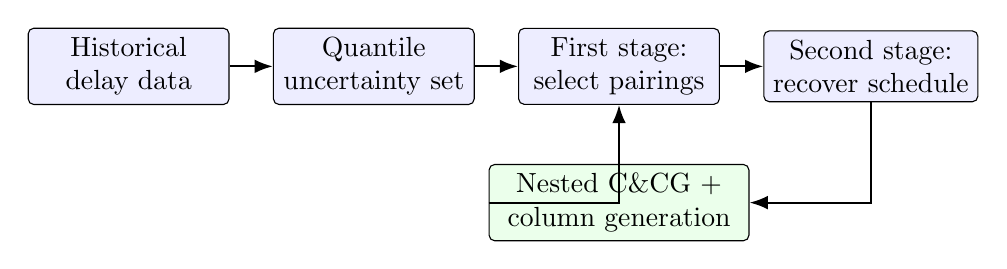
\begin{tikzpicture}[
    box/.style={draw, rounded corners=2pt, align=center, minimum width=2.55cm,
      minimum height=0.85cm, fill=blue!7},
    arrow/.style={-Latex, thick}
  ]
    \node[box] (data) {Historical\\delay data};
    \node[box, right=0.55cm of data] (uncertainty) {Quantile\\uncertainty set};
    \node[box, right=0.55cm of uncertainty] (master) {First stage:\\select pairings};
    \node[box, right=0.55cm of master] (recourse) {Second stage:\\recover schedule};

    \draw[arrow] (data) -- (uncertainty);
    \draw[arrow] (uncertainty) -- (master);
    \draw[arrow] (master) -- (recourse);

    \node[box, below=0.75cm of master, minimum width=3.3cm, fill=green!8] (alg)
      {Nested C\&CG +\\column generation};
    \draw[arrow] (recourse.south) |- (alg.east);
    \draw[arrow] (alg.west) -| (master.south);
  \end{tikzpicture}
  \end{center}

  \begin{itemize}
    \item First stage: choose feasible crew pairings.
    \item Second stage: minimize recovery cost under worst-case delays.
    \item Algorithm adds violated scenarios and negative-reduced-cost pairings.
  \end{itemize}
\end{frame}

% Speech note:
% The most important contribution is the re-optimization mechanism. When new
% delay data arrive, the uncertainty set may shrink or expand. If it shrinks,
% the old solution remains feasible and is simply conservative. If it expands,
% we can add new robustness cuts and re-optimize from the previous model,
% instead of rebuilding everything. In conclusion, this project aims to make
% crew pairing plans more robust, more data-driven, and easier to update when
% uncertainty changes. Thank you for listening.
\begin{frame}{Conclusion}
  \textbf{Main contribution: incremental re-optimization}

  \vspace{0.3cm}
  \begin{itemize}
    \item New data update the uncertainty bounds.
    \item If uncertainty shrinks, the previous robust plan remains feasible.
    \item If uncertainty expands, add new cuts and re-optimize.
    \item This avoids rebuilding the full model from zero.
  \end{itemize}

  \vspace{0.4cm}
  \begin{block}{Takeaway}
    The project designs a robust crew pairing method that learns from delay
    data and can adapt as uncertainty evolves.
  \end{block}
\end{frame}

\end{document}
